\documentclass[tikz,border=2pt]{standalone}
\usetikzlibrary{calc}
\usetikzlibrary{intersections}
\usetikzlibrary{patterns}
\usepackage{bm}
\usetikzlibrary{positioning}
\usetikzlibrary{shapes}
\usepackage{pgfplots}
\pgfplotsset{compat=1.18}

\begin{document}

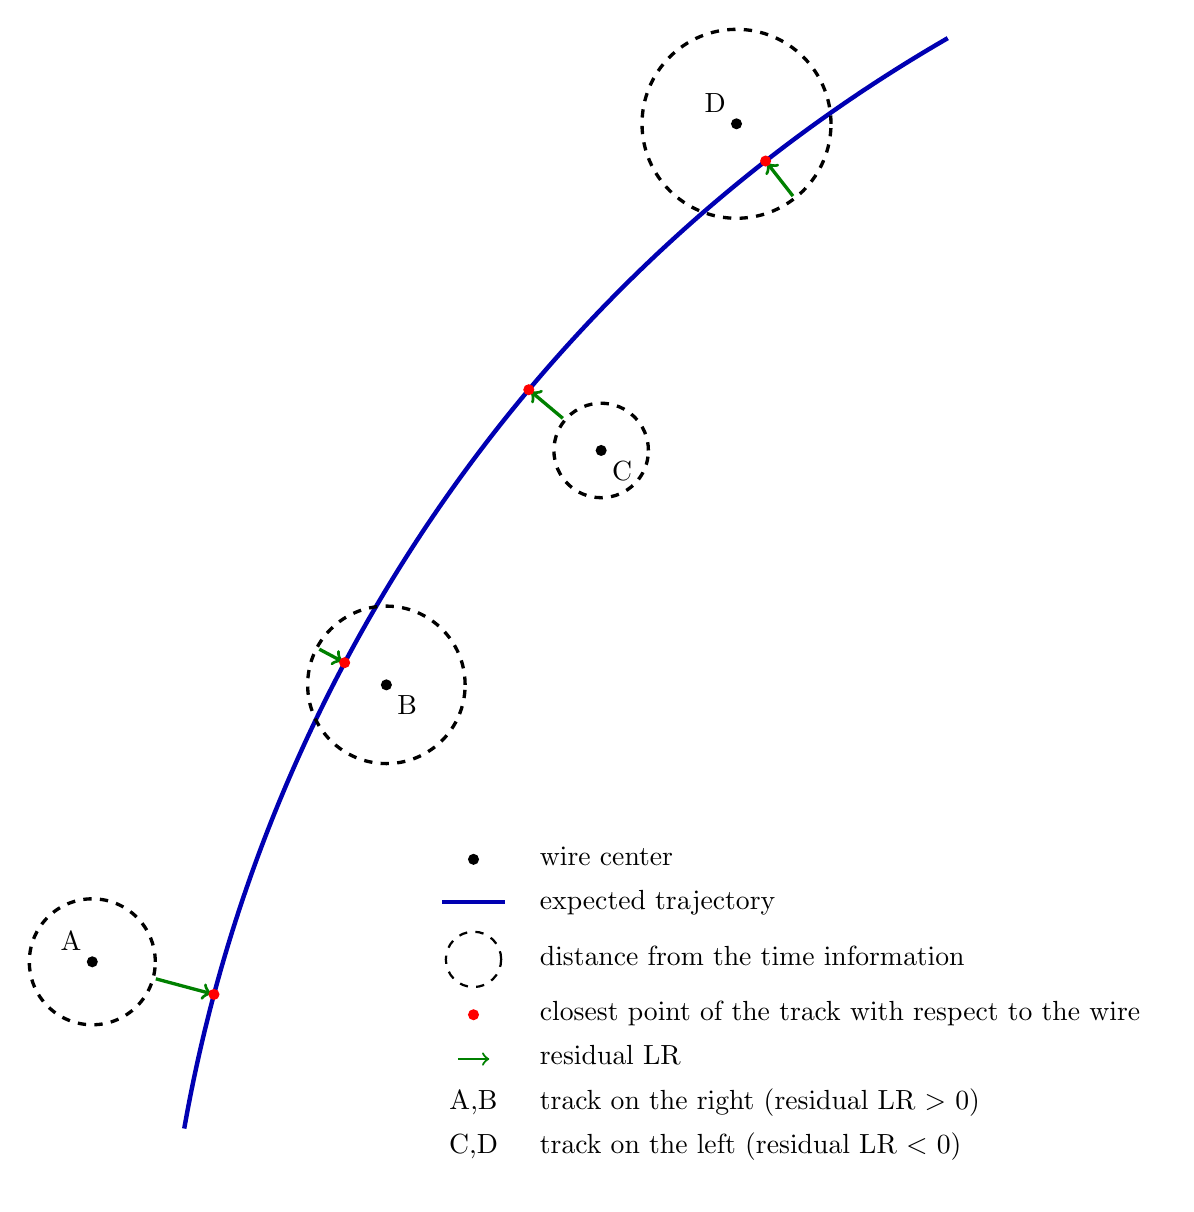
\begin{tikzpicture}[very thick]
    % \tikzset{
    %     every node/.style={font=\scriptsize}
    % }
    
    % ---- Notes ----
    % Track : portion of circle
    % Equation : y = 
    % 

    % Constants
    \pgfmathsetmacro{\xzero}{0}
    \pgfmathsetmacro{\yzero}{0}
    \pgfmathsetmacro{\R}{20}

    % Path
    \draw [ultra thick, blue!70!black] ($(\xzero, \yzero) + (170:\R)$) arc[radius=\R, start angle=170, end angle=120];

    % Control points
    \coordinate (O) at (\xzero, \yzero);
    \coordinate (A) at ($(O) + (165:\R)$);
    \coordinate (B) at ($(O) + (152:\R)$);
    \coordinate (C) at ($(O) + (140:\R)$);
    \coordinate (D) at ($(O) + (128:\R)$);

    % \fill (A) circle [radius=2pt];
    % \fill (B) circle [radius=2pt];
    % \fill (C) circle [radius=2pt];
    % \fill (D) circle [radius=2pt];

    % Points on the distance circles
    \coordinate (Ad) at ($(O)!1.08!(A)$);
    \coordinate (Bd) at ($(O)!0.97!(B)$);
    \coordinate (Cd) at ($(O)!0.94!(C)$);
    \coordinate (Dd) at ($(O)!1.03!(D)$);

    \draw [dashed] (Ad) circle [radius=0.04*\R];
    \fill (Ad) circle [radius=2pt];

    \draw [dashed] (Bd) circle [radius=0.05*\R];
    \fill (Bd) circle [radius=2pt];

    \draw [dashed] (Cd) circle [radius=0.03*\R];
    \fill (Cd) circle [radius=2pt];

    \draw [dashed] (Dd) circle [radius=0.06*\R];
    \fill (Dd) circle [radius=2pt];

    % correction arrows
    \draw [->,green!50!black, shorten <=1pt, shorten >=1pt] ($(O)!1.04!(A)$) -- (A);
    \draw [->,green!50!black, shorten <=1pt, shorten >=1pt] ($(O)!1.02!(B)$) -- (B);
    \draw [->,green!50!black, shorten <=1pt, shorten >=1pt] ($(O)!0.97!(C)$) -- (C);
    \draw [->,green!50!black, shorten <=1pt, shorten >=1pt] ($(O)!0.97!(D)$) -- (D);
    

    % Measurement points
    \fill [red] (A) circle [radius=2pt];
    \fill [red] (B) circle [radius=2pt];
    \fill [red] (C) circle [radius=2pt];
    \fill [red] (D) circle [radius=2pt];

    \node [above left] at (Ad) {A};
    \node [below right] at (Bd) {B};
    \node [below right] at (Cd) {C};
    \node [above left] at (Dd) {D};


    \newcommand{\solidline}{\raisebox{0.5ex}{\tikz \draw[thick] (0,0) -- (0.8,0);}}
    \newcommand{\dashedline}{\raisebox{0.5ex}{\tikz \draw[red, dashed, thick] (0,0) -- (0.8,0);}}
    
    \newcommand{\residualline}{\tikz[baseline=-0.5ex] \draw[green!50!black, thick,->] (0,0) -- (0.4,0);}
    \newcommand{\measurementpoint}{\tikz[baseline=-0.5ex] \fill[red] (0,0) circle [radius=2pt];}
    \newcommand{\wirepoint}{\tikz[baseline=-0.5ex] \fill (0,0) circle [radius=2pt];}
    \newcommand{\trackline}{\raisebox{0.5ex}{\tikz \draw[very thick,blue!70!black] (0,0) -- (0.8,0);}}
    \newcommand{\distanceline}{\tikz[baseline=-0.5ex] \draw[thick, dashed] (0,0) circle [radius=10pt];}

    \node at (-12,5) {
        \begin{tabular}{cl}
            \wirepoint  & wire center \\ [4pt]
            \trackline  & expected trajectory   \\[4pt]
            \distanceline   & distance from the time information  \\[8pt]
            \measurementpoint  & closest point of the track with respect to the wire  \\[4pt]
            \residualline   & residual LR \\ [4pt]
            A,B  & track on the right (residual LR $>$ 0)\\[4pt]
            C,D  & track on the left (residual LR $<$ 0)\\[4pt]

            
        \end{tabular}
    };


\end{tikzpicture}


\end{document}